
Im folgenden Abschnitt wird beschrieben, wie der betrachtete Datensatz in eine sinnvolle indizierbare Form
gebracht wird. Zunächst wird in \autoref{sec:preprosselection} ein
Überblick über die Auswahl der Fremdsoftware gegeben. Anschließend werden in
\autoref{sec:components} die einzelnen Schritte der Verarbeitung betrachtet.



\section{Auswahl}\label{sec:preprosselection}

Es existieren einige Toolboxen, die die Extraktion von Text und Meta-
Informationen vornehmen können.  Aufgrund der Wahl der
Programmiersprache Java wurde dazu das
\tika Toolkit
in Betracht gezogen. Es bietet einfach gestaltete Schnittstellen zu
Open Source Libraries um je nach Datenformat eine geeignete
Datenextraktion vorzunehmen. Neben PDFs lassen sich auch DOCs, Power
Point Präsentationen und Bilder mittels OCR ansprechen. Die Komponente der
PDF-Extraktion, \pdfbox, lässt sich auch außerhalb von Tika nutzen.
Die Paper-Auswahl besteht überwiegend aus PDFs\footnote{1595 PDFs,
  11 Docs und 1 HTML}, deswegen wurde \pdfbox ausgewählt, um einen-Overhead zu
vermeiden. Bei der Zunahme von weiteren Formaten lässt sich der Code
leicht mit entsprechenden \tika - Methoden austauschen.

Bei der Untersuchung des Datensatzes wird deutlich, dass nur ein
geringer Anteil an Papern korrekte Meta-Informationen angegeben werden. Um
Titel aus den Texten zu extrahieren wurde deswegen Docear
PdfDataExtractor\footnote{Link:
  \url{https://www.docear.org/tag/pdf-title-extraction/}}
eingesetzt. Die Software sucht, neben weitern Heuristiken, auf der
ersten Seite des Artikels nach langen zusammenhängenden Wortsequenzen.




\section{Komponenten}\label{sec:components}
In den folgenden Abschnitten werden die einzelnen Schritte der
Vorverarbeitung kurz dargelegt. Dabei liegt der Fokus auf der
Extraktion bzw. die Gewinnung der Meta-Daten.

\subsection{Meta-Daten-Extraktion}\label{sec:pdfextraction}

Sind die Daten extrahiert, so wird zunächst überprüft, ob der Titel der
Meta-Daten unzulässige Zeichen enthält oder eine unzulässige Länge
hat. Ist dies nicht der Fall, wird mit Docear PdfDataExtractor
versucht, im Text einen validen Titel zu finden. Valide Titel
werden an eine Schnittstelle der Digital Bibliography \& Library
Project (DBLP)\footnote{Link zu DBLP: \url{http://dblp.uni-trier.de/}}
gesendet und mit der dort vorliegenden Datenbank verglichen. Die Attribute des Artikels mit
der höchsten Übereinstimmung bzw. dem höchsten Score werden für den aktuellen
Artikel übernommen. Es besteht die Möglichkeit, den Datensatz als
XML-Datei lokal zu durchsuchen und mit weiteren Daten anzureichern.
In \autoref{sec:heuristic-title-search} soll weiter darauf
eingegangen werden.
Konnte nach wie vor kein valider Titel entnommen
werden, wird eine Zeichenkette festgelegter Länge als Heuristik für
den Title angenommen. In diesem Fall wird eine Named Entity
Recognition auf den ersten Wörtern des Artikel-Textes gefahren, um mögliche
Autoren zu finden. Hierzu wird Apache OpenNLP verwendet\footnote{Link zu
  OpenNLP: \url{https://opennlp.apache.org/}}.

Aufgrund der vergleichsweise geringen Anzahl an Papern werden die
Artikel-Daten einzeln als XML-Files gespeichert. Das erleichtert die
Überprüfung während der Entwicklungsphase. Das Haupt-Element
article enthält die Elemente 
\begin{itemize}
\item metaData mit title, authors, publificationDate, refCount und
\item textElements mit abstract und fullText. 
\end{itemize}

Um die von der ASCII Codierung abweichende Zeichen korrekt darzustellen,
werden die Text-Elemente  als nicht interpretierte Zeichen gespeichert.
Zusätzlichen werden fileName, filePath sowie parseTime festgehalten,
die in der weiteren Verarbeitung benötigt werden. 

\subsection{Heuristische Titel Suche}\label{sec:heuristic-title-search}

Die extrahierten Daten zeigen auch nach den in \autoref{sec:pdfextraction}
beschriebenen Schritten ein nicht zufriedenstellendes Ergebnis. Im folgenden soll eine heuristische
Titel Suche vorgestellt werden\footnote{Vorschlag: Martin Potthast.}, die den Text mit Attributen einer
vorliegenden Meta-Daten Kollektion vergleicht. Der Algorithmus
folgt der Annahme, dass die Meta-Daten mit der höchsten Übereinstimmung
die korrekten sein müssen, wenn diese als Vergleichsdaten
vorliegen. Als Daten-Quelle wurde zum einen eine Auswahl an Papern des DBLP, die in relevanten Journalen erscheinen und eine bereits vorhandene Auswertung von
Zitations-Analysen\footnote{wie zitiere ich denn den Herren?}
zusammengefasst. Der Algorithmus durchläuft je extrahiertem 
Artikel die folgende Prozedur:

Eine vorgegebene Anzahl an Wörtern des Artikels wird als zu
vergleichender Text gespeichert. Während der Stax-Parser über die
Meta-Daten-Kollektion läuft, werden die Elemente als aktuelles 
Artikel-Objekt gespeichert. Es wird ein Score berechnet, der eine
mögliche Übereinstimmung anzeigen soll. Enthält der entsprechende Text Wörter der
Attribute Titel, Autoren oder Publikations-Zeitpunkt, erhält der Artikel Punkte. Genaue Übereinstimmung des
Titels bzw. der Autoren erhalten zusätzliche Boni, die relativ zur
Länge der Attribute berechnet werden. Die Bewertung für korrekte Titel mit 50 und Autoren mit 30 brachte hier akzeptable Ergebnisse. Der Artikel mit der höchsten Punktzahl wird akzeptiert. Da
nicht garantiert werden kann, dass die korrekte Artikel Daten gefunden
werden, muss der Score einen Schwellwert überschreiten.

\subsection{Ranking der Dokumente}\label{sec:ranking}

%\subsubsection{Paperrank}\label{sec:paperrank}

Die gegebenen Paper können auch zur Indizierungszeit gerankt werden. Hierbei spielt die Relevanz zu einer Query noch keine Rolle. Es geht darum, welches Paper generell wichtiger ist, als ein anderes. Diese Gewichtung wird in das finale Ranking einberechnet.
Es existieren diverse Faktoren nach denen die Relevanz von Papers im Bezug auf andere Papers festgemacht werden kann. Im Zuge der Bearbeitung wurden zum Einen die Anzahl der Klicks und die Verweildauer auf einem Paper einbezogen und zum Anderen die Zahl der Zitierungen in anderen Papers. Weitere Faktoren, wie bspw. Autoren, Sprache oder Form wurden für das Ranking nicht hinzugezogen, könnten jedoch in weiteren Arbeiten zu dem Thema betrachtet werden.  \\

In diesem Abschnitt wird auf die Anzahl der Zitierungen für jedes Paper eingegangen. In Anlehnung an den Begriff Pagerank wird dies hier als Paperrank bezeichnet.
Webseiten nehmen Bezug auf andere Webseiten. Es ist möglich daran die Wichtigkeit einer Webseite festzumachen. Wird eine oft auf anderen Seiten erwähnt ist davon auszugehen, dass sie wichtiger ist, als eine weniger erwähnte. Bei Papers ist das ähnlich: Wird ein Paper oft zitiert so ist davon auszugehen, dass es für die Autoren von Papers eine höhere Relevanz hat, als Papers die weniger zitiert werden. Daher wurde dieser Aspekt für das Ranking der Dokumente für die Suchmaschine betrachtet. Außerdem kann als Nebeneffekt anhand des Paperranks die komplette Verteilung der Zitierungen dargestellt werden.
Die Umsetzung erfolgte über ein Perlskript, es gab Probleme bei der Umsetzung mit Java. Das Skript kann Offline zur Indexing-Zeit ausgeführt werden. Es wird vom Hauptprogramm über die Javaklasse \lstinline{RunScript.class} aufgerufen. Das Skript wurde für die Perl Version 5 getestet\footnote{Hier bitte die Readme beachten.}. Das Skript wurde zur besseren Nachvollziehbarkeit in einzelne Schritte unterteilt auf die im Folgenden eingegangen wird.
Zunächst wurden zur Feststellung einige Grunddaten aus den gegebenen wissenschaftlichen Texten benötigt. Daraus wurden im speziellen die Titel und die Quellen genutzt. Die Paper liegen dank der Vorverarbeitung in Form von Textdateien vor. Die Titel sind durch die XML-Tag <title> markiert. Es erfolgte eine Extraktion durch reguläre Ausdrücke auf den <title>-Tag und zur Sicherheit, da nicht alle Paper einen ordentlich befüllten Tag hatten auf den <Filename>-Tag. 
Die erste Herausforderung stellte die Extraktion der Quellen für jedes Paper dar. Diese sind nicht gesondert markiert, sondern sind im Text eingebettet. Dies wurde mit Hilfe einer Heuristik gelöst. Quellen sind typischer Weise nummeriert. Diese Nummerierung wird oftmals eingeschlossen durch eckige [] oder runde () Klammern. Daher wurde mit Hilfe regulärer Ausdrücke nach Klammern gesucht, welche ein- oder zweistellige Zahlen enthalten. War diese Bedingung erfüllt, wurde die entsprechende Zeile als Quelle extrahiert. Mit diesen Daten für Titel und Quellen wurde nun weitergearbeitet.
Im nächsten Schritt werden die so entstandenen Quellen in Zeichenketten zerlegt. Für eine Länge von 30 Zeichen haben sich gute Ergebnisse eingestellt. Dies geschieht, da die Quellen nicht nur den Titel der zitierten Quelle enthalten, sondern auch Dinge wie bspw. Erscheinungsdatum, Author, Verlag, ISBN. 
Danach können die Zeichenketten mit den Titeln abgeglichen werden. Wenn der Titel die Zeichenkette beinhaltet, dann wird der Titel in den nächsten Bearbeitungsschritt übernommen. Hierbei werden beim Abgleich Sonderzeichen und Zahlen ausgenommen\footnote{escaped}.
Daraufhin werden die Titel gezählt und sortiert. Es entsteht eine Liste mit den Papers zusammen mit der Anzahl mit der sie in den Quellen der anderen Paper vorkommen. Daraus kann nun entnommen werden, welche Paper die wichtigsten sind. Die Datei wurde in ein XML-File umgewandelt um eine reibungslose Weiterverarbeitung zu gewährleisten. Außerdem wurde die Datei, durch entfernen von unnötigen Leerzeichen etc., etwas bereinigt, um Speicherplatz einzusparen und eine höhere Effizienz zu gewährleisten. Das Ergebnis ist in \autoref{fig:paperrank} dargestellt:


%%%


\begin{figure}[ht]

    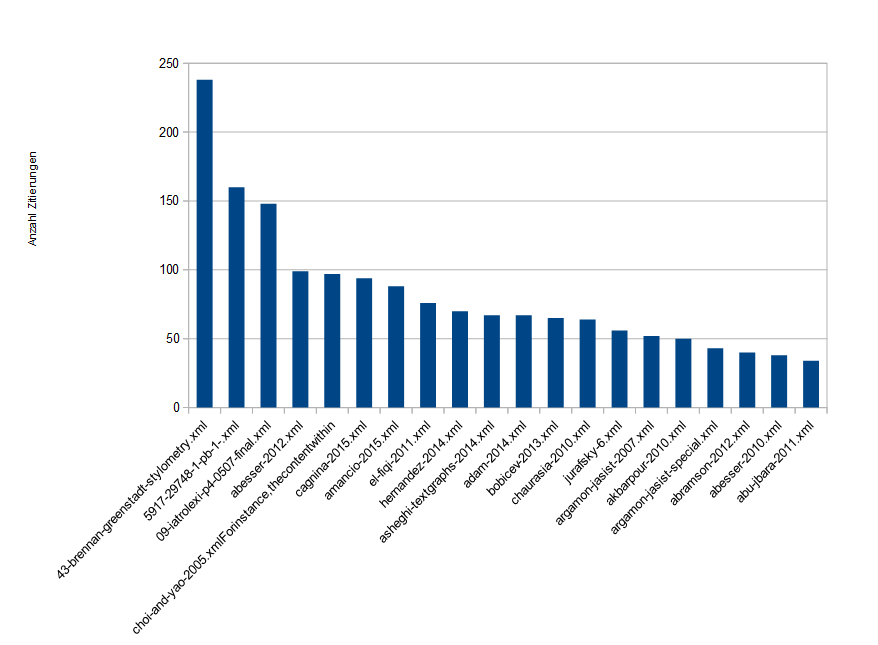
\includegraphics[width=\linewidth]{anzahl_zitierungen}
  \caption[]{Anzahl der Zitierungen für die top 20 Paper}
\label{fig:paperrank}
\end{figure}



Zum Abschluss wurden die entsprechenden gezählten Zitierungen in die Ausgangsdateien geschrieben. Sie wurden in <entry>- und <counter>-Tags verpackt, damit im Scoring Schritt ein reibungsloser Zugriff möglich wird.
Nun soll noch ein kurzer Ausblick gegeben werden, was nicht in das Resultat des Paperranks eingeflossen ist, aber die Ergebnisse noch verbessern könnte. Bei der Extraktion der Quellen ist sicher noch einiges an Optimierungspotenzial. Es könnten weitere Kriterien in die Auswahl einfließen, um zum einen mehr Quellen zu finden und zum anderen \emph{Nichtquellen} zu eliminieren. Außerdem wurde nicht beachtet, welche Quelle die Zitierungen vornimmt. Generell hat sich das Vorgehen an keinem Algorithmus, wie bspw. dem Random Surfer Modell orientiert. Dies wäre auch ein interessanter Ansatz für weitere Nachforschungen. 
Nichtsdestotrotz entstand mit dieser Arbeit eine weitere Möglichkeit die gegebenen wissenschaftlichen Texte zu bewerten bzw. zu \emph{ranken}. Des Weiteren ist nun eine Aussage darüber möglich, wie oft einzelne Paper in anderen Papern als Quellen herangezogen werden und wie die  Verteilung über alle Texte ist.



%%% Local Variables:
%%% mode: latex
%%% TeX-master: "../arbeit"
%%% End:
